\documentclass[UTF8]{article}
\usepackage{graphicx}
\usepackage{subfigure}
\usepackage{amsmath}
\usepackage{makecell}
\usepackage[utf8]{inputenc}
\usepackage[space]{ctex} %中文包
\usepackage{listings} %放代码
\usepackage{xcolor} %代码着色宏包
\usepackage{CJK} %显示中文宏包
\usepackage{float}
\usepackage{makecell}
\usepackage{diagbox}
\usepackage{bm}
\usepackage{ulem} 
\usepackage{amssymb}
\usepackage{soul}
\usepackage{color}
\usepackage{geometry}
\usepackage{fancybox} %花里胡哨的盒子
\usepackage{xhfill} %填充包, 可画分割线 https://www.latexstudio.net/archives/8245
\usepackage{multicol} %多栏包
\usepackage{enumerate} %可以方便地自定义枚举标题
\usepackage{multirow} %表格中多行单元格合并
\usepackage{wasysym} %可以使用wasysym里的一堆奇奇怪怪的符号
\usepackage{tikz}
\usepackage{tikZ-timing} % 时序图支持
\usetikzlibrary{arrows,shapes,automata,petri,positioning,calc}
\usetikzlibrary{shadows} % 阴影支持
\usepackage[colorlinks,linkcolor=red]{hyperref} % 超链接支持

\geometry{left = 1.5cm, right = 1.5cm, top=2cm, bottom=2cm}

\definecolor{mygreen}{rgb}{0,0.6,0}
\definecolor{mygray}{rgb}{0.5,0.5,0.5}
\definecolor{mymauve}{rgb}{0.58,0,0.82}
\lstset{
	backgroundcolor=\color{white}, 
	%\tiny < \scriptsize < \footnotesize < \small < \normalsize < \large < \Large < \LARGE < \huge < \Huge
	basicstyle = \footnotesize,       
	breakatwhitespace = false,        
	breaklines = true,                 
	captionpos = b,                    
	commentstyle = \color{mygreen}\bfseries,
	extendedchars = false,
	frame = shadowbox, 
	framerule=0.5pt,
	keepspaces=true,
	keywordstyle=\color{blue}\bfseries, % keyword style
	language = C++,                     % the language of code
	otherkeywords={string}, 
	numbers=left, 
	numbersep=5pt,
	numberstyle=\tiny\color{mygray},
	rulecolor=\color{black},         
	showspaces=false,  
	showstringspaces=false, 
	showtabs=false,    
	stepnumber=1,         
	stringstyle=\color{mymauve},        % string literal style
	tabsize=4,          
	title=\lstname           
}

%\sum\nolimits_{j=1}^{M}   上下标位于求和符号的水平右端,
%\sum\limits_{j=1}^{M}   上下标位于求和符号的上下处,
%\sum_{j=1}^{M}  对上下标位置没有设定,会随公式所处环境自动调整。

%%%%%%%%%%%%%画图包%%%%%%%%%%%%%
\usepackage{tikz}
%%%%%%%%%%%%%好看的矩形%%%%%%%%%%%%%
\tikzset{
  rect1/.style = {
    shape = rectangle,% 指定样式
    minimum height=2cm,% 最小高度
    minimum width=4cm,% 最小宽度
    align = center,% 文字居中
    drop shadow,% 阴影
  }
}
%%%%%%%%%%%%%画图背景包%%%%%%%%%%%%%
\usetikzlibrary{backgrounds}

%%%%%%%%%%%%%在tikz中画一个顶点%%%%%%%%%%%%%
%%%%%%%%%%%%%#1:node名称%%%%%%%%%%%%%
%%%%%%%%%%%%%#2:位置%%%%%%%%%%%%%
%%%%%%%%%%%%%#3:标签%%%%%%%%%%%%%
\newcommand{\newVertex}[3]{\node[circle, draw=black, line width=1pt, scale=0.8] (#1) at #2{#3}}
%%%%%%%%%%%%%在tikz中画一条边%%%%%%%%%%%%%
\newcommand{\newEdge}[2]{\draw [black,very thick](#1)--(#2)}
%%%%%%%%%%%%%在tikz中放一个标签%%%%%%%%%%%%%
%%%%%%%%%%%%%#1:名称%%%%%%%%%%%%%
%%%%%%%%%%%%%#2:位置%%%%%%%%%%%%%
%%%%%%%%%%%%%#3:标签内容%%%%%%%%%%%%%
\newcommand{\newLabel}[3]{\node[line width=1pt] (#1) at #2{#3}}

%%%%%%%%%%%%%强制跳过一行%%%%%%%%%%%%%
\newcommand{\jumpLine} {\hspace*{\fill} \par}
%%%%%%%%%%%%%关键点指令,可用itemise替代%%%%%%%%%%%%%
\newcommand{\average}[1]{\left\langle #1\right\rangle }
%%%%%%%%%%%%%表格内嵌套表格%%%%%%%%%%%%%
\newcommand{\keypoint}[2]{$\bullet$\textbf{#1}\quad#2\par}
%%%%%%%%%%%%%<T>平均值表示%%%%%%%%%%%%%
\newcommand{\tabincell}[2]{\begin{tabular}{@{}#1@{}}#2\end{tabular}}%放在导言区
%%%%%%%%%%%%%大黑点item头%%%%%%%%%%%%%
\newcommand{\itemblt}{\item[$\bullet$]}
%%%%%%%%%%%%%大圈item头%%%%%%%%%%%%%
\newcommand{\itemc}{\item[$\circ$]}
%%%%%%%%%%%%%大星星item头%%%%%%%%%%%%%
\newcommand{\itembs}{\item[$\bigstar$]}
%%%%%%%%%%%%%右▷item头%%%%%%%%%%%%%
\newcommand{\itemrhd}{\item[$\rhd$]}
%%%%%%%%%%%%%定义为%%%%%%%%%%%%%
\newcommand{\defas}{=_{df}}
%%%%%%%%%%%%%蕴含%%%%%%%%%%%%%
\newcommand{\imp}{\rightarrow}

%%%%%%%%%%%%%双线分割线%%%%%%%%%%%%%
\newcommand*{\doublerule}{\hrule width \hsize height 1pt \kern 0.5mm \hrule width \hsize height 2pt}
%%%%%%%%%%%%%双线中间可加东西的分割线%%%%%%%%%%%%%
\newcommand\doublerulefill{\leavevmode\leaders\vbox{\hrule width .1pt\kern1pt\hrule}\hfill\kern0pt }
%%%%%%%%%%%%%左大括号%%%%%%%%%%%%%
\newcommand{\leftbig}[1]{\left\{\begin{array}{l}#1\end{array}\right.}
%%%%%%%%%%%%%矩阵%%%%%%%%%%%%%
\newcommand{\mat}[2]{\left[\begin{array}{#1}#2\end{array}\right]}
%%%%%%%%%%%%%可换行圆角文本框%%%%%%%%%%%%%

\newcommand{\ovalboxn}[1]{\ovalbox{\tabincell{l}{#1}}}
%%%%%%%%%%%%%设置section的counter, 使从0开始%%%%%%%%%%%%%

\title{软件工程导论 HW1}
\date{}
\author{PB18111697 王章瀚}

\begin{document}
\maketitle
\section{}
\subsection{用例图}
\begin{figure}[H]
	\centering
	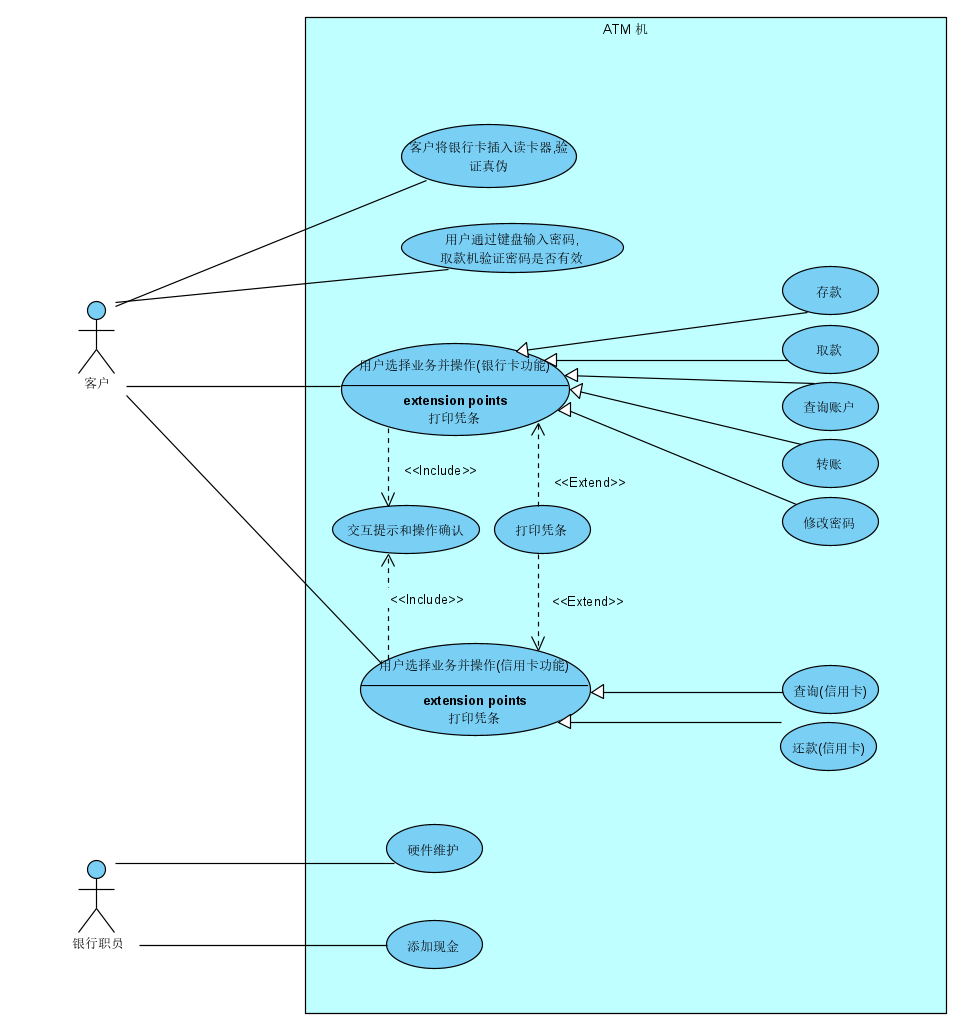
\includegraphics[width=\linewidth]{1.png}
	\caption{题 1 的用例图}
\end{figure}\par
\subsection{用例表}
\subsubsection{用例: 客户将银行卡插入读卡器,验证真伪}
\noindent
\textbf{用例}: 客户将银行卡插入读卡器验证真伪
\\
\textbf{目标}: 验证银行卡的真伪
\\
\textbf{前提条件}: 无
\\
\textbf{触发器}: 用户插入卡
\\
\textbf{场景}: \\
	\hspace*{2em} 用户使用 ATM 机器 \\
\textbf{异常}: \\
	\hspace*{2em} 无法识别银行卡 \\
%\textbf{优先级}: 
%\\
\textbf{何时可用}: ATM 营业时间
\\
\textbf{使用频率}: 每次用户操作都会使用
\\
\textbf{使用方式}:\\
	\hspace*{2em}1. 用户插入银行卡 \\
	\hspace*{2em}2. ATM 机验证真伪 \\
\textbf{扩展点}: 无
\\
\textbf{次要参与者}: 无
\\
\textbf{次要参与者使用方式}: 无
\\
\textbf{未解决的问题}: \\
	\hspace*{2em}1. 对于无法识别的银行卡应作何反应?
	

\subsubsection{用例: 用户通过键盘输入密码, 取款机验证密码是否有效}
\noindent
\textbf{用例}: 用户通过键盘输入密码, 取款机验证密码是否有效
\\
\textbf{目标}: 验证银行卡密码是否正确以确定身份
\\
\textbf{前提条件}: 用例 "插入银行卡" 已完成
\\
\textbf{触发器}: 用户操作输入密码验证身份
\\
\textbf{场景}: \\
	\hspace*{2em} 用户使用 ATM 机器进行相关操作 \\
\textbf{异常}: \\
	\hspace*{2em} 用户密码输入错误 \\
%\textbf{优先级}: 
%\\
\textbf{何时可用}: 用户插入卡后
\\
\textbf{使用频率}: 用户首次插入银行卡后验证
\\
\textbf{使用方式}:\\
	\hspace*{2em}1. 用户通过键盘输入银行卡密码 \\
	\hspace*{2em}2. ATM 机验证真伪 \\
\textbf{扩展点}: 无
\\
\textbf{次要参与者}: 无
\\
\textbf{次要参与者使用方式}: 无
\\
\textbf{未解决的问题}: \\
	\hspace*{2em}1. 对于无法识别的银行卡应作何反应?
	
\subsubsection{用例: 用户选择业务并操作(银行卡功能)——存款}
\noindent
\textbf{用例}: 用户选择业务并操作(银行卡功能)
\\
\textbf{目标}: 完成用户的操作需求
\\
\textbf{前提条件}: 用例 "插入银行卡" 和 用例 "验证密码" 已完成
\\
\textbf{触发器}: 用户选择了存款操作
\\
\textbf{场景}: \\
	\hspace*{2em}1. 用户选择存款操作 \\
	\hspace*{2em}2. 根据屏幕信息的交互提示进行操作确认 \\
	\hspace*{2em}3. 用户放入纸钞 \\
	\hspace*{2em}4. 系统验证可识别纸钞数目 \\
	\hspace*{2em}5. 完成操作 \\
	\hspace*{2em} 5. 用户可以选择是否打印凭条 \\
\textbf{异常}: \\
	\hspace*{2em} 1. 存款时, 用户放入纸钞有问题——重新执行 \\
	\hspace*{2em} 2. 凭条打印用纸不足——让银行职员处理 \\
%\textbf{优先级}: 
%\\
\textbf{何时可用}: 用户插入银行卡并完成密码验证后
\\
\textbf{使用频率}: 一天多次
\\
\textbf{使用方式}: 根据屏幕信息的交互提示进行操作确认等
\\
\textbf{扩展点}: \\
	\hspace*{2em}1. 打印凭条 \\
\textbf{次要参与者}: 银行职员
\\
\textbf{次要参与者使用方式}: 直接打开 ATM 机箱操作.
\\
\textbf{未解决的问题}: \\
	\hspace*{2em} 1. 凭条打印纸不足时如何通知银行职员处理? \\
	
\subsubsection{用例: 用户选择业务并操作(银行卡功能)——取款}
\noindent
\textbf{用例}: 用户选择业务并操作(银行卡功能)
\\
\textbf{目标}: 完成用户的操作需求
\\
\textbf{前提条件}: 用例 "插入银行卡" 和 用例 "验证密码" 已完成
\\
\textbf{触发器}: 用户选择了取款操作
\\
\textbf{场景}: \\
	\hspace*{2em}1. 用户选择取款操作 \\
	\hspace*{2em}2. 根据屏幕信息的交互提示进行操作确认 \\
	\hspace*{2em}3. 系统吐出纸钞 \\
	\hspace*{2em}4. 用户拿走纸钞 \\
	\hspace*{2em}5. 完成操作 \\
	\hspace*{2em} 5. 用户可以选择是否打印凭条 \\
\textbf{异常}: \\
	\hspace*{2em} 1. 纸钞不足——让银行职员添加现金 \\
	\hspace*{2em} 2. 凭条打印用纸不足——银行职员提供设备维护 \\
%\textbf{优先级}: 
%\\
\textbf{何时可用}: 用户插入银行卡并完成密码验证后
\\
\textbf{使用频率}: 一天多次
\\
\textbf{使用方式}: 根据屏幕信息的交互提示进行操作确认等
\\
\textbf{扩展点}: \\
	\hspace*{2em}1. 打印凭条 \\
\textbf{次要参与者}: 银行职员
\\
\textbf{次要参与者使用方式}: 直接打开 ATM 机箱操作.
\\
\textbf{未解决的问题}: \\
	\hspace*{2em} 1. 纸钞不足时如何通知银行职员处理? \\
	\hspace*{2em} 2. 凭条打印纸不足时如何通知银行职员处理? \\
		
\subsubsection{用例: 用户选择业务并操作(银行卡功能)——查询账户}
\noindent
\textbf{用例}: 用户选择业务并操作(银行卡功能)
\\
\textbf{目标}: 完成用户的操作需求
\\
\textbf{前提条件}: 用例 "插入银行卡" 和 用例 "验证密码" 已完成
\\
\textbf{触发器}: 用户选择了查询账户操作
\\
\textbf{场景}: \\
	\hspace*{2em}1. 用户选择查询账户操作 \\
	\hspace*{2em}2. 根据屏幕信息的交互提示进行操作确认 \\
	\hspace*{2em}3. 用户确认后退出 \\
	\hspace*{2em} 5. 用户可以选择是否打印凭条 \\
\textbf{异常}: 无 \\
%\textbf{优先级}: 
%\\
\textbf{何时可用}: 用户插入银行卡并完成密码验证后
\\
\textbf{使用频率}: 一天多次
\\
\textbf{使用方式}: 根据屏幕信息的交互提示进行操作确认等
\\
\textbf{扩展点}: \\
	\hspace*{2em}1. 打印凭条 \\
\textbf{次要参与者}: 银行职员
\\
\textbf{次要参与者使用方式}: 直接打开 ATM 机箱操作.
\\
\textbf{未解决的问题}: \\
	\hspace*{2em} 1. 凭条打印纸不足时如何通知银行职员处理? \\
			
\subsubsection{用例: 用户选择业务并操作(银行卡功能)——修改密码}
\noindent
\textbf{用例}: 用户选择业务并操作(银行卡功能)
\\
\textbf{目标}: 完成用户的操作需求
\\
\textbf{前提条件}: 用例 "插入银行卡" 和 用例 "验证密码" 已完成
\\
\textbf{触发器}: 用户选择了修改密码操作
\\
\textbf{场景}: \\
	\hspace*{2em}1. 用户选择修改密码操作 \\
	\hspace*{2em}2. 根据屏幕信息的交互提示进行操作确认 \\
	\hspace*{2em}3. 用户确认后退出 \\
	\hspace*{2em}5. 用户可以选择是否打印凭条 \\
\textbf{异常}: 无
%\textbf{优先级}: 
%\\
\textbf{何时可用}: 用户插入银行卡并完成密码验证后
\\
\textbf{使用频率}: 一天多次
\\
\textbf{使用方式}: 根据屏幕信息的交互提示进行操作确认等
\\
\textbf{扩展点}: \\
	\hspace*{2em}1. 打印凭条 \\
\textbf{次要参与者}: 无
\\
\textbf{次要参与者使用方式}: 无
\\
\textbf{未解决的问题}: 无
	
	
\subsubsection{用例: 用户选择业务并操作(信用卡功能)——查询}
\noindent
\textbf{用例}: 用户选择业务并操作(信用卡功能)
\\
\textbf{目标}: 完成用户的操作需求
\\
\textbf{前提条件}: 用例 "插入银行卡" 和 用例 "验证密码" 已完成
\\
\textbf{触发器}: 用户选择查询操作
\\
\textbf{场景}: \\
	\hspace*{2em} 1. 用户需要查询信用卡 \\
	\hspace*{2em} 2. 系统显示信用卡相关信息 \\
	\hspace*{2em} 3. 用户退出 \\
	\hspace*{2em} 5. 用户可以选择是否打印凭条 \\
\textbf{异常}: \\
	\hspace*{2em} 1. 信用卡资料缺失——让客户到人工柜台处理 \\
	\hspace*{2em} 2. 凭条打印用纸不足——让银行职员添加 \\
%\textbf{优先级}: 
%\\
\textbf{何时可用}: 用户插入银行卡并完成密码验证后
\\
\textbf{使用频率}: 一天多次
\\
\textbf{使用方式}: 根据屏幕信息的交互提示进行操作确认等 \\
\textbf{扩展点}: \\
	\hspace*{2em}1. 打印凭条 \\
\textbf{次要参与者}: 银行职员
\\
\textbf{次要参与者使用方式}: 直接打开 ATM 机箱操作.
\\
\textbf{未解决的问题}: \\
	\hspace*{2em} 1. 凭条打印纸不足时如何通知银行职员处理? \\
		
		
\subsubsection{用例: 用户选择业务并操作(信用卡功能)——还款}
\noindent
\textbf{用例}: 用户选择业务并操作(信用卡功能)
\\
\textbf{目标}: 完成用户的操作需求
\\
\textbf{前提条件}: 用例 "插入银行卡" 和 用例 "验证密码" 已完成
\\
\textbf{触发器}: 用户选择还款操作
\\
\textbf{场景}: \\
	\hspace*{2em} 1. 用户需要还款信用卡 \\
	\hspace*{2em} 2. 系统显示信用卡相关信息 \\
	\hspace*{2em} 3. 用户放入纸钞或选择还款金额 \\
	\hspace*{2em} 4. 系统确认并返回信息 \\
	\hspace*{2em} 5. 用户可以选择是否打印凭条 \\
	
\textbf{异常}: \\
	\hspace*{2em} 1. 用户纸钞额不足或余额不足——让用户重新选择还款金额 \\
	\hspace*{2em} 2. 凭条打印用纸不足——让银行职员添加 \\
%\textbf{优先级}: 
%\\
\textbf{何时可用}: 用户插入银行卡并完成密码验证后
\\
\textbf{使用频率}: 一天多次
\\
\textbf{使用方式}: 根据屏幕信息的交互提示进行操作确认等 \\
\textbf{扩展点}: \\
	\hspace*{2em}1. 打印凭条 \\
\textbf{次要参与者}: 银行职员
\\
\textbf{次要参与者使用方式}: 直接打开 ATM 机箱操作.
\\
\textbf{未解决的问题}: \\
	\hspace*{2em} 1. 凭条打印纸不足时如何通知银行职员处理? \\
			
			
\subsubsection{用例: 银行职员进行设备维护}
\noindent
\textbf{用例}: 银行职员进行设备维护
\\
\textbf{目标}: 维护 ATM 系统设备
\\
\textbf{前提条件}: 无
\\
\textbf{触发器}: 无
\\
\textbf{场景}: \\
	\hspace*{2em} 1. 银行职员打开 ATM 机箱进行维护
\textbf{异常}: 无
%\textbf{优先级}: 
%\\
\textbf{何时可用}: 无用户正在进行 ATM 操作时
\\
\textbf{使用频率}: 一天一次
\\
\textbf{使用方式}: 直接对 ATM 机箱进行操作 \\
\textbf{扩展点}: 无
\\
\textbf{次要参与者}: 无
\\
\textbf{次要参与者使用方式}: 无
\\
\textbf{未解决的问题}: 无
			
			
\subsubsection{用例: 银行职员添加现金}
\noindent
\textbf{用例}: 银行职员添加现金
\\
\textbf{目标}: 为 ATM 系统添加现金
\\
\textbf{前提条件}: 无
\\
\textbf{触发器}: 无
\\
\textbf{场景}: \\
	\hspace*{2em} 1. 银行职员打开 ATM 机箱 \\
	\hspace*{2em} 2. 银行职员放入现金 \\
\textbf{异常}: 无
%\textbf{优先级}: 
%\\
\textbf{何时可用}: 无用户正在进行 ATM 操作时
\\
\textbf{使用频率}: 一天一次
\\
\textbf{使用方式}: 直接对 ATM 机箱进行操作 \\
\textbf{扩展点}: 无
\\
\textbf{次要参与者}: 无
\\
\textbf{次要参与者使用方式}: 无
\\
\textbf{未解决的问题}: 无
		
\newpage
\section{2}
\subsection{用例图}
\begin{figure}[H]
	\centering
	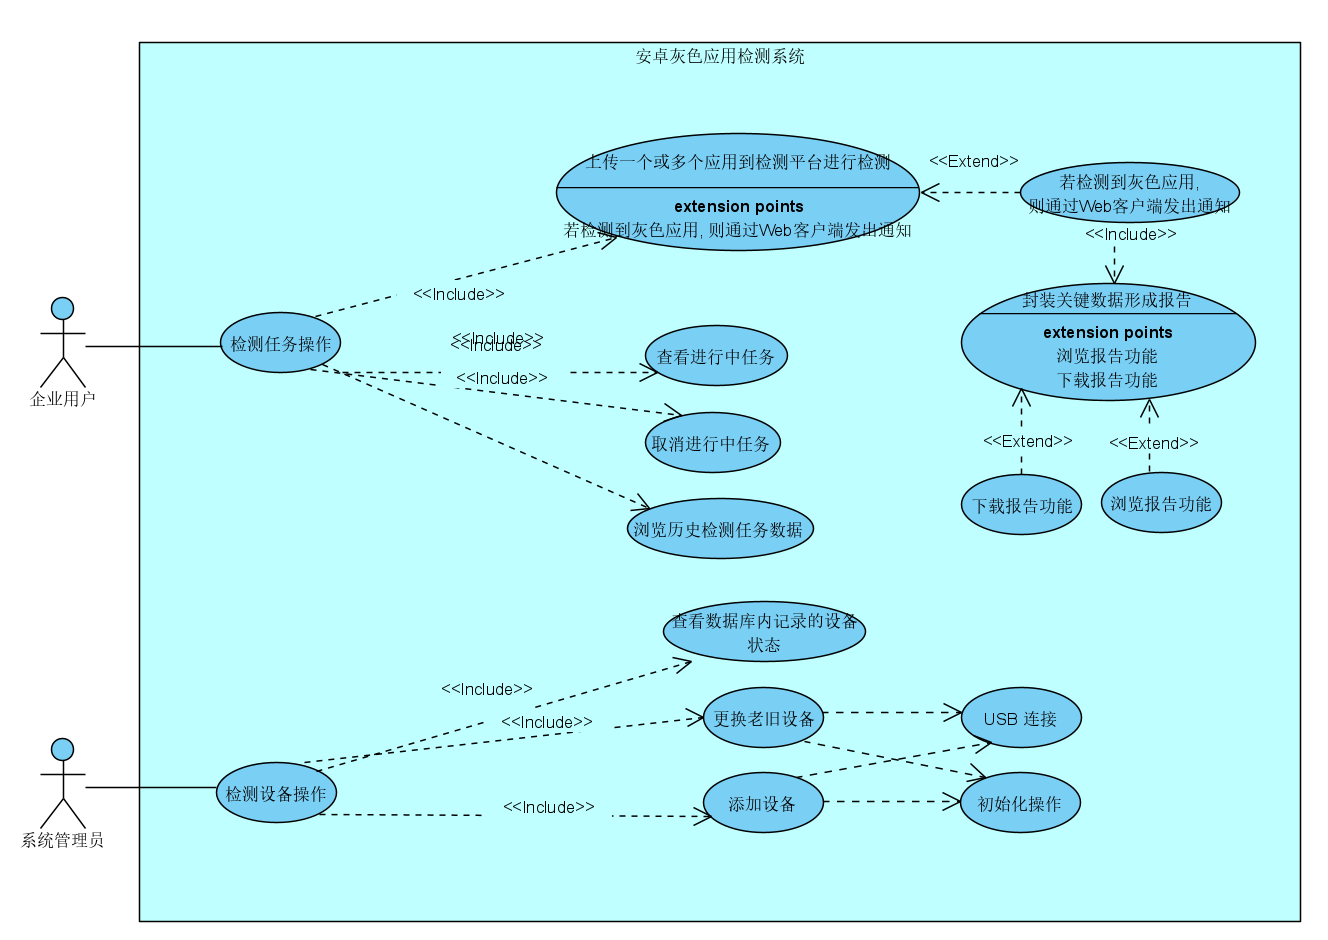
\includegraphics[width=\linewidth]{2.png}
	\caption{题 2 的用例图}
\end{figure}\par
\subsection{用例表}
\subsubsection{用例: 企业用户上传应用到检测平台检测}
\noindent
\textbf{用例}: 企业用户上传应用到检测平台检测
\\
\textbf{目标}: 检测应用是否为灰色应用
\\
\textbf{前提条件}: 无
\\
\textbf{触发器}: 企业用户提交
\\
\textbf{场景}: \\
	\hspace*{2em} 1. 企业用户上传一个或多个应用到检测平台 \\
	\hspace*{2em} 2. 若检测平台检测到灰色应用, 就封装相关的关键数据形成报告, 通过 web 客户端发送通知给用户 \\
	\hspace*{2em} 3. 客户端提供下载报告功能 \\
	\hspace*{2em} 4. 客户端提供浏览报告功能 \\
\textbf{异常}: \\
	\hspace*{2em} 1. 应用有问题, 无法检测——通知客户 \\
%\textbf{优先级}: 
%\\
\textbf{何时可用}: 任何时候
\\
\textbf{使用频率}: 一月多次
\\
\textbf{使用方式}: 企业用户通过客户端进行操作 \\
\textbf{扩展点}: \\
	\hspace*{2em} 1. 通知发送 \\
	\hspace*{2em} 2. 浏览报告 \\
	\hspace*{2em} 3. 下载报告 \\
\\
\textbf{次要参与者}: 无
\\
\textbf{次要参与者使用方式}: 无
\\
\textbf{未解决的问题}: \\
	\hspace*{2em} 1. 以何种格式向客户端返回报告信息? \\
	\hspace*{2em} 2. 如何管理与存储用户查询记录和相关报告等? \\
	
\subsubsection{用例: 企业用户查看进行中任务}
\noindent
\textbf{用例}: 企业用户查看进行中任务
\\
\textbf{目标}: 查看进行中的任务状态
\\
\textbf{前提条件}: 已有进行中任务
\\
\textbf{触发器}: 企业用户触发查询
\\
\textbf{场景}: \\
	\hspace*{2em} 1. 平台列出进行中任务 \\
	\hspace*{2em} 2. 用户选择任务 \\
	\hspace*{2em} 3. 平台返回任务相关信息 \\
\textbf{异常}: \\
	\hspace*{2em} 1. 任务信息暂不可得——用户等待 \\
%\textbf{优先级}: 
%\\
\textbf{何时可用}: 任何时候
\\
\textbf{使用频率}: 一月多次
\\
\textbf{使用方式}: 企业用户通过客户端进行操作 \\
\textbf{扩展点}: 无
\\
\textbf{次要参与者}: 无
\\
\textbf{次要参与者使用方式}: 无
\\
\textbf{未解决的问题}: \\
	\hspace*{2em} 1. 以何种格式向客户端返回报告信息? \\
	\hspace*{2em} 1. 以何种格式列出进行中任务? \\
		
\subsubsection{用例: 企业用户取消进行中任务}
\noindent
\textbf{用例}: 企业用户取消进行中任务
\\
\textbf{目标}: 取消进行中的任务状态
\\
\textbf{前提条件}: 已有进行中任务
\\
\textbf{触发器}: 企业用户触发取消功能
\\
\textbf{场景}: \\
	\hspace*{2em} 1. 平台列出进行中任务 \\
	\hspace*{2em} 2. 用户选择要取消的任务 \\
	\hspace*{2em} 3. 平台返回取消操作是否成功 \\
\textbf{异常}: \\
	\hspace*{2em} 1. 任务因各种原因不可取消——提供客服等给用户 \\
%\textbf{优先级}: 
%\\
\textbf{何时可用}: 任何时候
\\
\textbf{使用频率}: 一月多次
\\
\textbf{使用方式}: 企业用户通过客户端进行操作 \\
\textbf{扩展点}: 无
\\
\textbf{次要参与者}: 无
\\
\textbf{次要参与者使用方式}: 无
\\
\textbf{未解决的问题}: \\
	\hspace*{2em} 1. 什么样才算是成功取消? \\
	\hspace*{2em} 2. 取消后的记录如何保存? \\
			
\subsubsection{用例: 企业用户浏览历史检测任务数据}
\noindent
\textbf{用例}: 企业用户浏览历史检测任务数据
\\
\textbf{目标}: 查看进行中的任务状态
\\
\textbf{前提条件}: 无
\\
\textbf{触发器}: 企业用户触发查询功能
\\
\textbf{场景}: \\
	\hspace*{2em} 1. 平台列出历史任务 \\
	\hspace*{2em} 2. 用户选择任务 \\
	\hspace*{2em} 3. 平台返回任务对应数据 \\
\textbf{异常}: \\
	\hspace*{2em} 1. 历史数据不存在等——让用户确认 \\
%\textbf{优先级}: 
%\\
\textbf{何时可用}: 任何时候 \\
\textbf{使用频率}: 一月多次 \\
\textbf{使用方式}: 企业用户通过客户端进行操作 \\
\textbf{扩展点}: 无 \\
\textbf{次要参与者}: 无 \\
\textbf{次要参与者使用方式}: 无 \\
\textbf{未解决的问题}: 
	\hspace*{2em} 1. 历史数据丢失如何处理? \\
	\hspace*{2em} 2. 用户找不到想要的历史记录怎么办? \\
	\hspace*{2em} 3. 什么样的查询方式更好, 仅基于时间顺序不一定最优? \\
				
\subsubsection{用例: 系统管理员查看数据库内记录的设备状态}
\noindent
\textbf{用例}: 系统管理员查看数据库内记录的设备状态
\\
\textbf{目标}: 检查系统是否有问题
\\
\textbf{前提条件}: 无
\\
\textbf{触发器}: 系统管理员触发查询
\\
\textbf{场景}: \\
	\hspace*{2em} 1. 系统管理员输入查询代码 \\
	\hspace*{2em} 2. 系统返回查询结果 \\
\textbf{异常}: 无 \\
%\textbf{优先级}: 
%\\
\textbf{何时可用}: 任何时候 \\
\textbf{使用频率}: 一月一次 \\
\textbf{使用方式}: 系统管理员打开系统管理界面操作 \\
\textbf{扩展点}: 无 \\
\textbf{次要参与者}: 无 \\
\textbf{次要参与者使用方式}: 无 \\
\textbf{未解决的问题}: 无 \\
				
\subsubsection{用例: 系统管理员更换老旧设备}
\noindent
\textbf{用例}: 系统管理员更换老旧设备
\\
\textbf{目标}: 将老旧设备更换为新设备
\\
\textbf{前提条件}: 无
\\
\textbf{触发器}: 系统管理员需要更换老旧设备
\\
\textbf{场景}: \\
	\hspace*{2em} 1. 系统管理员移除旧设备, 接入新设备 \\
	\hspace*{2em} 2. 系统管理员通过 USB 连接 \\
	\hspace*{2em} 3. 系统管理员完成初始化操作 \\
\textbf{异常}: \\
	\hspace*{2em} 1. 系统无法识别新设备——尝试换用其他新设备 \\
%\textbf{优先级}: 
%\\
\textbf{何时可用}: 任何时候 \\
\textbf{使用频率}: 一年多次 \\
\textbf{使用方式}: 系统管理员打开机箱更换设备, 并通过控制面板操作 \\
\textbf{扩展点}: 无 \\
\textbf{次要参与者}: 无 \\
\textbf{次要参与者使用方式}: 无 \\
\textbf{未解决的问题}: 无 \\
				
\subsubsection{用例: 系统管理员添加新设备}
\noindent
\textbf{用例}: 系统管理员添加新设备
\\
\textbf{目标}: 为系统添加新设备
\\
\textbf{前提条件}: 无
\\
\textbf{触发器}: 系统管理员需要添加新设备
\\
\textbf{场景}: \\
	\hspace*{2em} 1. 系统管理员接入新设备 \\
	\hspace*{2em} 2. 系统管理员通过 USB 连接 \\
	\hspace*{2em} 3. 系统管理员完成初始化操作 \\
\textbf{异常}: \\
	\hspace*{2em} 1. 系统无法识别新设备——尝试换用其他新设备 \\
	\hspace*{2em} 2. 设备槽已满——不允许再添加 \\
%\textbf{优先级}: 
%\\
\textbf{何时可用}: 任何时候 \\
\textbf{使用频率}: 一年多次 \\
\textbf{使用方式}: 系统管理员打开机箱添加设备, 并通过控制面板操作 \\
\textbf{扩展点}: 无 \\
\textbf{次要参与者}: 无 \\
\textbf{次要参与者使用方式}: 无 \\
\textbf{未解决的问题}: 无 \\
	

\end{document}


